\documentclass{article}

%\usepackage{biblatex} %Imports biblatex package
%\usepackage[sorting=none, backend=bibtex]{biblatex}
%]{biblatex}
\usepackage[
    backend=biber, 
    natbib=true,
    style=ieee,
    sorting=none
]{biblatex}
\addbibresource{bibliography.bib} %Import the bibliography file


\usepackage{graphicx,wrapfig,lipsum}
%\usepackage{ucs}
\usepackage[utf8]{inputenc}
\usepackage[main=greek,english]{babel}
\newcommand{\en}{\selectlanguage{english}}
\newcommand{\gr}{\selectlanguage{greek}}

\title{Η επιρροή των κοινωνικών δικτύων στην καθημερινότητα}


\author{Στυλιανάκης Στυλιανός \\
Κωστόπουλος Κωνσταντίνος Παναγιώτης \\
Κονταράκης Ιωάννης Γεώργιος
}

\date{\today}
\addto{\captionsgreek}{\renewcommand{\abstractname}{Περίληψη - 249 Λέξεις}}

\begin{document}
\maketitle  
\begin{abstract}
Στις μέρες μας, τα κοινωνικά δίκτυα αποτελούν αναπόσπαστο κομμάτι της καθημερινότητάς μας. Παρόλα αυτά, κατά τη χρήση τους ελλοχεύουν πολλοί κίνδυνοι, οι οποίοι είναι αναγκαίο να μελετώνται συνεχώς και εκτενώς, ώστε να υπάρξει προσπάθεια ελάττωσής τους. Έρευνες έχουν αποδείξει ότι η κατάθλιψη, η επιβολή πολιτικού προσανατολισμού και η παραπληροφόρηση αποτελούν τρεις από τις πιο συνηθισμένες επιδράσεις που ταλανίζουν όλο και πιο συχνά το κοινό των πλατφορμών αυτών. Η συνεχής σύγκριση των χρηστών με τον ουτοπικό τρόπο ζωής που προβάλουν οι φίλοι τους, τους οδηγεί συχνά σε απογοήτευση για την «απλή» και «βαρετή» ζωή τους. Μόνο εάν ο χρήστης αντιληφθεί τον κίνδυνο αυτό μπορεί καταφέρει να μην επηρεάζεται αρνητικά από τέτοιου είδους αναρτήσεις. Ένα άλλο φαινόμενο το οποίο θα πρέπει να γνωρίζει είναι η προώθηση συγκεκριμένων πολιτικών αναρτήσεων από τους αλγορίθμους εξατομίκευσης. Έχει αποδειχθεί ότι συγκεκριμένες πολιτικές παρατάξεις προβάλλονται πιο συχνά από ότι άλλες, γεγονός το οποίο μπορεί να χειραγωγήσει τον πολιτικό προσανατολισμό κάποιων χρηστών. Εκτός από πολιτικά μηνύματα, τα κοινωνικά δίκτυα πολλές φορές μπορούν να προωθήσουν και άλλου είδους πληροφορίες για τις οποίες, για προφανείς λόγους, δεν έχει προηγηθεί κάποια επικύρωση της εγκυρότητάς τους. Αυτή η αφιλτράριστη επανεμφάνιση αναρτήσεων είναι αυτό που καθιστά τα κοινωνικά δίκτυα επιρρεπή στη διάδοση παραπληροφόρησης. Είναι λοιπόν προφανές ότι παρόλες τις ευκολίες που μας παρέχουν οι πλατφόρμες κοινωνικής δικτύωσης, πολλές φορές κρύβουν κινδύνους για τους χρήστες τους, οι οποίοι έχουν την υποχρέωση να φιλτράρουν το περιεχόμενο που καταναλώνουν σε αυτές. Αυτοί είναι οι κίνδυνοι που στη συνέχεια εξετάζονται σε εμβάθυνση στις παρακάτω παρατιθέμενες μελέτες.
\end{abstract}
\clearpage 
\tableofcontents
\section{Βιβλιογραφική Παρουσίαση - 893 Λέξεις}
Η ψυχική υγεία είναι ένας σημαντικός παράγοντας στη ζωή του ατόμου, ικανή να επηρεάσει πολλές πτυχές της. Αυτό έχει οδηγήσει στην πραγματοποίηση εκτεταμένων ερευνών γύρω από το θέμα, ένα μεγάλο ποσοστό των οποίων επικεντρώνεται στην ευτυχία, η οποία είναι άρρηκτα συνδεδεμένη με την ψυχική υγεία. Μία διαδικασία που μπορεί να επηρεάσει την ευτυχία του ατόμου είναι η κοινωνικοποίηση. Στις μέρες μας, περίοπτη θέση στη διαδικασία αυτή έχουν τα κοινωνικά δίκτυα.

Την επίδραση αυτή των δικτύων εξερευνά και το άρθρο των \en Neha Mundada\gr  και \en Vinit Parakh \parencite{article7}\gr, στο οποίο εξετάζεται μία παραλλαγή του παραδόξου της φιλίας. Το παράδοξο της φιλίας αναφέρει ότι «κατά μέσο όρο, οι φίλοι σου έχουν πιο πολλούς φίλους από εσένα». Αυτό συμβαίνει επειδή υπάρχει μεγάλη πιθανότητα κάποιος να έχει έναν «δημοφιλή» φίλο, ο οποίος να ανεβάζει το μέσο όρο. Η παραλλαγή που εξετάζεται ισχυρίζεται ότι «Οι φίλοι σου είναι πιο χαρούμενοι από εσένα».

Οι αρθρογράφοι στηρίζουν την υπόθεση αυτή στο γεγονός ότι το μεγαλύτερο ποσοστό των αναρτήσεων στα κοινωνικά δίκτυα έχει θετικό περιεχόμενο. Η έκθεση των ενεργών χρηστών σε τέτοιου είδους αναρτήσεις, προκαλεί μία ψευδαίσθηση ευτυχίας των φίλων τους. Αυτή στη συνέχεια πυροδοτεί μία υποσυνείδητη σύγκριση της πραγματικής ζωής του χρήστη με την ψευδαίσθηση αυτή, οδηγώντας τους έτσι στη δυστυχία.
Χρησιμοποιώντας αναρτήσεις από το \en Twitter\gr, οι ερευνητές έφτασαν στο συμπέρασμα ότι το παράδοξο της ευτυχίας ισχύει για περίπου 73-79\% των χρηστών της πλατφόρμας, ανάλογα τη μετρική που θα ληφθεί υπόψιν. Ταυτόχρονα, εξετάστηκε και το αντίθετο παράδοξο «Οι φίλοι σου είναι πιο λυπημένοι από σένα» όπου ίσχυε για το 20-23\% των χρηστών. Κλείνοντας, οι ερευνητές υπενθυμίζουν στους αναγνώστες ότι αν λυπούνται επειδή οι φίλοι τους φαντάζουν πιο χαρούμενοι από τους ίδιους στα κοινωνικά δίκτυα, βρίσκονται στην ίδια κατάσταση με την πλειοψηφία των χρηστών των πλατφορμών αυτών.


Εκτός από την επιρροή στην ψυχική υγεία των ατόμων, τα κοινωνικά δίκτυα είναι ικανά να κατευθύνουν και τον πολιτικό προσανατολισμό τους. Αυτήν την υπόθεση ερευνά και το άρθρο \en “Algorithmic amplification of politics on Twitter’’ \parencite{article9}\gr , το οποίο εξετάζει την προώθηση των πολιτικών αναρτήσεων από τους αλγορίθμους του \en Twitter \gr. Είναι γνωστό πως η επιλογή, καθώς και η σειρά εμφάνισης αναρτήσεων στην αρχική σελίδα των χρηστών της πλατφόρμας καθορίζεται από αλγορίθμους εξατομίκευσης. Συνεπώς, οι αλγόριθμοι αυτοί έχουν τη δυνατότητα τόσο να ενισχύσουν, όσο και να καταστείλουν πολιτικά μηνύματα, ανάλογα με τη συχνότητα και τη σειρά εμφάνισής τους στις αρχικές σελίδες των χρηστών. 
Η έρευνα χωρίζεται σε δύο κομμάτια, το πρώτο από τα οποία εξετάζει αναρτήσεις μελών πολιτικών κομμάτων από επτά διαφορετικές χώρες και καταλήγει στο συμπέρασμα ότι, σε έξι από αυτές, τα κυρίαρχα δεξιά κόμματα προωθούνται πιο συχνά από τους αλγορίθμους σε σχέση με τα κυρίαρχα αριστερά. Αντίστοιχα, το δεύτερο σκέλος της έρευνας πραγματεύεται Αμερικανικά ειδησεογραφικά μέσα, αποκαλύπτοντας μία παρόμοια προτίμηση των αλγορίθμων για δεξιοστρεφή μέσα. 
Τέλος, μελετά εάν υπάρχει παραπάνω αλγοριθμική προώθηση για ακροδεξιά και ακροαριστερά κόμματα σε σχέση με τα πιο κεντρικά, καταρρίπτοντας όμως στη συνέχεια τη θεωρία αυτή.

Πέρα από την ταλάντευση του πολιτικού προσανατολισμού, τα μέσα κοινωνικής δικτύωσης, λόγω της ελευθερίας του λόγου που προσφέρουν, βοηθάνε στην εύκολη και γρήγορη διάδοση πληροφοριών, ανεξαρτήτως της εγκυρότητάς τους.  Έτσι, πολλές φορές αποτελούν πομπό διάδοσης παραπληροφόρησης, όπως εξετάζεται στη μελέτη των \en Hunt Allcott , Matthew Gentzkow \gr και \en Chuan Yu\parencite{article4}. \gr Πιο συγκεκριμένα, οι συγγραφείς αναφέρουν πως στις μέρες μας η παραπληροφόρηση στα μέσα δικτύωσης μαστίζει τις κοινωνίες και τα δημοκρατικά καθεστώτα. Το 2016 ομάδα Αμερικανών εξέθεσε ψεύτικες προεκλογικές έρευνες, κάτι που επηρέασε την κοινή γνώμη στις εκλογές του 2016. Για τον λόγο αυτό το \en Facebook \gr και άλλα κοινωνικά δίκτυα προσπάθησαν να ελαττώσουν το κύκλωμα της παραπληροφόρησης.  Πράγμα που κατάφερε το \en Facebook \gr πιθανώς εξαιτίας της νέας πλατφόρμας του, η οποία προσπαθεί να συνδράμει στον περιορισμό της παραπληροφόρησης . Παρόλα αυτά, σύμφωνα με το κείμενο , το ποσοστό της παραπληροφόρησης στο \en Facebook \gr παραμένει υψηλό . Έπειτα αναφέρονται κάποια δεδομένα και αποτελέσματα για την παραπληροφόρηση γενικά στα μέσα.
Τέλος, η διάδοση της παραπληροφόρησης είναι μία πιθανή απειλή για τις κοινωνίες και την δημοκρατία. Ωστόσο, μετά την αλλαγή πλατφόρμας στο  \en Facebook \gr η παραπληροφόρηση έχει μειωθεί δραματικά ενώ στο \en Twitter \gr συνεχίζει να αυξάνεται.

Μία άλλη παρεμφερής έρευνα που έχει υλοποιηθεί περί του θέματος είναι και αυτή του \en Jason Hong \parencite{article1}\gr, ο οποίος τοποθετείται για το πώς οι επιστήμονες της τεχνολογίας μπορούν να βοηθήσουν στα προβλήματα των κοινωνικών δικτύων (παραπληροφόρηση, επιτήδεια και μη). Αρχικά,  θεωρεί πως το \en Facebook \gr θα πρέπει να συμπεριλάβει αλγορίθμους περιορισμού για την καταπολέμηση των παραπάνω προβλημάτων , κάτι όμως που δεν θα λειτουργούσε αφού οι αλγόριθμοι του είναι αρκετά πολύπλοκοι. Οι αλγόριθμοι μπορεί να χρησιμοποιούν διάφορες παραμέτρους οι οποίες δεν συσχετίζονται άμεσα με την παραπληροφόρηση. Σύμφωνα με ερευνητές οι αλγόριθμοι του \en Facebook \gr λειτουργούν ως επί τω πλείστων βάση δημοτικότητας , κάτι το οποίο οδηγεί στην παραπληροφόρηση κυρίως για πολιτικά θέματα. Παρόλα αυτά, είναι αδύνατο να μπλοκάρεις αναρτήσεις χρηστών εξαιτίας υψηλής δημοτικότητας αφού δεν ανήκουν όλες οι αναρτήσεις στις “προβληματικές’’. Το \en Facebook \gr αναφέρει πως είχε λάβει μέτρα ασφαλείας στις εκλογές του 2020 και φαίνεται πως τα μέτρα αυτά απέδωσαν και έτσι ο \en Jason Hong \gr αναρωτιέται τον λόγο για τον οποίο δεν είναι σε ισχύ. Στο κείμενο αναφέρεται πως αν οι αλγόριθμοι του \en Facebook \gr λειτουργούσαν με άλλο τρόπο πέρα από την δημοτικότητα των αναρτήσεων τα κοινωνικά μέσα δικτύωσης θα ήταν εντελώς διαφορετικά , με θετικά αποτελέσματα. Το \en Facebook \gr έχει ανάγκη από ερευνητές για να τροποποιήσουν τους αλγορίθμους για την αποφυγή των προαναφερθέντων προβλημάτων.
\section{Βιβλιογραφία}

\en{\printbibliography[heading=none]} %Prints bibliography
\nocite{*}

\gr\section{Υπόμνημα}
\subsection{Ομάδα - 95 Λέξεις}
Αρχικά, υλοποιήσαμε την ενότητα “Επιλογή Άρθρων’’ όλοι μαζί, μοιράσαμε τα έξι επιλεγμένα άρθρα και ο καθένας ανέλαβε δύο από αυτά. Στη συνέχεια, τα μελετήσαμε, γράψαμε μία περίληψη για το καθένα και αφού τελειώσαμε τη διαδικασία αυτή διαβάσαμε όλοι τις περιλήψεις των συνεργατών μας. Έπειτα, αποφασίσαμε ποια άρθρα θα συμπεριληφθούν στη Βιβλιογραφική μας Παρουσίαση και συνεργαστήκαμε στη συγγραφή των ενοτήτων “Εξαίρεση άρθρων’’ και “Βιβλιογραφική Παρουσίαση’’. Στη συνέχεια, ανατέθηκε μία από τις υπόλοιπες ενότητες (Περίληψη, Ομάδα, Παρουσίαση) στον καθένα. Τέλος, ο καθένας έγραψε τη δικιά του “Χρυσή Παράγραφο’’ και όλοι μαζί βιντεοσκοπήσαμε την παρουσίαση.

\subsection{Επιλογή Άρθρων}
Επώνυμα: ΚΟΝΤΑΡΑΚΗΣ ΚΩΣΤΟΠΟΥΛΟΣ ΣΤΥΛΙΑΝΑΚΗΣ
\newline\en
SHA-1: \textbf{479}0bb9bf\textbf{8}bc07c7\textbf{a}809\textbf{1}2d2123e694e9a21d1f2
\newline \gr
Διακριτά ψηφία: 4, 7, 9, 8, \en a, 1\gr

\subsection{Εξαίρεση Άρθρων - 150 Λέξεις}
Τα άρθρα 9 – \en “Humans rely more on algorithms than social influence as a task becomes more difficult’’ \gr και \en a – “Resolution of the Happiness–Income Paradox’’ \gr δεν αναφέρονται στην επιρροή των κοινωνικών μέσων δικτύωσης στην καθημερινότητα. Για τον λόγο αυτό δεν συμπεριλήφθηκαν στην περίληψη μας, με τίτλο “Η επιρροή των κοινωνικών δικτύων στην καθημερινότητα”. Πιο συγκεκριμένα το άρθρο 4 αναφέρεται στην επιρροή των αλγορίθμων στην λήψη αποφάσεων και καταλήγει στο ότι το κοινό προτιμά την επίλυση ενός προβλήματος μέσω ενός αλγορίθμου, παρά την άποψη του κοινού, όσο το πρόβλημα γίνεται πιο πολύπλοκο. Από την άλλη, το άρθρο  a αναφέρεται στην ευτυχία του ατόμου και κυρίως στη σχέση του εισοδήματος με την ευτυχία. Στο άρθρο υποστηρίζεται πως αν και το εισόδημα παίζει πρωταρχικό ρόλο στην ευτυχία του ατόμου, σημαντικό ρόλο παίζουν και άλλοι παράγοντες, όπως η ατομική υγεία, η σχέση με την οικογένεια, η διασκέδαση και η εργασία.

\section{Βιογραφικά}
\subsection*{Στυλιανάκης Στυλιανός - 69 Λέξεις}
\begin{wrapfigure}{l}{2cm}
	
\includegraphics[width=2cm]{Stylianakis.jpg}
\end{wrapfigure} 
Ο Στυλιανάκης Στυλιανός γεννήθηκε την 1η Φεβρουαρίου του 1999 στα Χανιά της Κρήτης. Σπουδάζει στο Τμήμα Μηχανικών Υπολογιστών και Πληροφορικής του Πανεπιστημίου Πατρών, στο οποίο και εισήχθη το Σεπτέμβριο του 2017. Είναι απόφοιτος γενικού λυκείου και έχει άπταιστη γνώση της αγγλικής γλώσσας, για την οποία κατέχει δίπλωμα C2. Κύρια χαρακτηριστικά του αποτελούν η υπομονή, το ομαδικό πνεύμα, καθώς και η αγάπη για το αντικείμενο των Ηλεκτρονικών Υπολογιστών. 

\subsection*{Κωστόπουλος Κωνσταντίνος Παναγιώτης - 57 Λέξεις}
\begin{wrapfigure}{r}{2cm}
	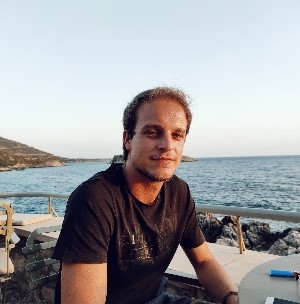
\includegraphics[width=2cm]{Kostopoulos.jpg}
\end{wrapfigure} 
Ο Κωνσταντίνος-Παναγιώτης Κωστόπουλος γεννημένος την 30η Ιανουαρίου του 2000 στο Ρίο Πατρών. Είναι φοιτητής στο Πανεπιστήμιο Πατρών στο Τμήμα Μηχανικών Ηλεκτρονικών Υπολογιστών και Πληροφορικής \en(CEID) \gr, στο οποίο εισήχθη τον Οκτώβριο του 2018. Είναι απόφοιτος γενικού λυκείου και μιλά άψογα την αγγλική γλώσσα . Διακατέχεται από όρεξη για μάθηση, είναι ευγενικός, επικοινωνιακός και ομαδικός.

\subsection*{Κονταράκης Ιωάννης Γεώργιος - 58 Λέξεις}
\begin{wrapfigure}{l}{2cm}
	
\includegraphics[width=2cm]{Kontarakis.jpg}
\end{wrapfigure} 
Ο Ιωάννης Γεώργιος Κονταράκης γεννημένος στα Χανιά Κρήτης στις 17 Ιούλιου του 1999, εντάχθηκε στο τμήμα μηχανικών υπολογιστών του πανεπιστημίου Πατρών το 2019. Του αρέσει πολύ το αντικείμενο των υπολογιστών, αφού ασχολείται από πολύ μικρή ηλικία. Κατέχει πτυχίο \en proficiency \gr αγγλικών και έχει όρεξη για μάθηση. Του αρέσει ο συναγωνισμός, είναι υπομονετικός και ορίζει συνεχώς νέους στόχους.

\end{document}